\section{Specifying Counting Networks}
\label{sec:counting}

We now show how to use subjective histories to specify another class
of non-linearizable objects---\emph{counting networks}.
%
Counting networks are a special case of \emph{balancing networks}
introduced by Aspnes \etal~\cite{Aspnes-al:JACM94}, themselves
building on sorting networks~\cite{Ajtai-al:STOC83}, aimed to
implement concurrent counters in a way free from synchronization
bottlenecks.
%
The key idea is to decompose the workload between \emph{several}
counters, so that each of them is responsible for a disjoint set of
values. A thread trying to increment first approaches the
\emph{balancer}, which is a logical ``switch'' that ``directs'' the
thread, \ie, provides it with the address of the counter to increment.
%
The balancers make counting networks' operations
\emph{non-linearizable}, as in the presence of interference the
results of increments might be observed out of order.
%
% \wrt~a sequential specification.
{
%\setlength{\belowcaptionskip}{-15pt} 
\begin{figure}%[18]{r}{4cm} 
\begin{tabular}{c@{\ \ \ \ \ \ }c}
\begin{minipage}[c]{2.5cm}
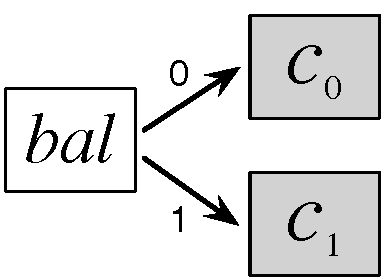
\includegraphics[width=2.1cm]{counter.pdf} 
\end{minipage}
&
\begin{minipage}[l]{4.9cm}
\centering
{\small{
\[
\begin{array}{rl}
\Num{1} & \esc{getAndInc()} : \esc{nat}~=~\esc{\{}  \\[2pt] 
\Num{2} & ~~~~ b \Asgn \esc{flip(}\bal\esc{)};\\[2pt]
\Num{3} & ~~~~ \res \Asgn \esc{fetchAndAdd2(}c_b\esc{)};\\[2pt]
\Num{4} & ~~~~ \kw{return}~\res~\esc{\}}
\end{array}
\]
}}
\end{minipage} 
%
\end{tabular}
%
\vspace{-10pt}  
\caption{Simple counting network}
\label{fig:counter-fig} 
%\vspace{-15pt}  
\end{figure}
}

Figure~\ref{fig:counter-fig} presents a schematic outline and a
pseudo-code implementation of a counting network with a single
balancer.
%
The implementation contains three pointers: the balancer $\bal$, which
stores either 0 or 1, thus directing threads to the shared pointers
$c_0$ or $c_1$, which count the even and odd values,
respectively. Threads increment by calling \code{getAndInc}, which
works as follows. It first atomically changes the bit value of the
balancer via a call to atomic operation \code{flip} (line 2). The
\code{flip} operation returns the \emph{previous} value $b$ of the
balancer as a result, thus determining which of the counters, $c_0$ or
$c_1$, should be incremented. The thread proceeds to atomically add 2
to the value of $c_b$ via \code{fetchAndAdd2} (line 3). The old value
of $c_b$ is returned as the result of the procedure.\footnote{In the
  counting network from Figure~\ref{fig:counter-fig}, the balancer
  itself might seem like a contention point. However, the \code{flip}
  operation is much less expensive than \code{CAS} as a
  synchronization mechanism. The performance can be further improved
  by constructing a \emph{diffracting tree} of several
  balancers~\cite[\S 12.6]{Herlihy-Shavit:08}, but we do not consider
  diffracting trees here.}

Assuming that $c_0$ and $c_1$ are initialized with $0$ and $1$, it is
easy to see that in a single-threaded program, the network will behave
as a conventional counter; that is, consecutive invocations of
\code{getAndInc} return consecutive nats.
%
However, in the concurrent setting, \code{getAndInc} may return
results out of order, as follows. 
%
% which historically led to the definition of quiescent
% consistency~\cite[\S 3.3]{Herlihy-Shavit:08} in order to specify the
% network's concurrent behavior.

\vspace{3pt}
\begin{example}
\label{ex:t1t2}
%
Consider two threads, $T_1$ and $T_2$ operating on the network
initialized with $\bal\,{\mapsto}\,0$, $c_b\,{\mapsto}\,b$. $T_1$
calls \code{getAndInc} and executes its line~2 to set $\bal$ to 1. It
gets suspended, so $T_2$ proceeds to execute lines~2 and~3, therefore
setting $\bal$ back to $0$ and returning $1$. While $T_1$ is still
suspended, $T_2$ calls \code{getAndInc} again, gets directed to $c_0$,
and returns 0, after it has just returned 1.
%
\end{example}
\vspace{3pt}

\noindent

This out-of-order behavior, however, is not random, and can be
precisely characterized as a function of the number of threads
operating on the
network~\cite{Afek-al:OPODIS10,Jagadeesan-Riely:ICALP14}. In the rest
of this section and in Section~\ref{sec:qclients}, we show how to
capture such bounds in the spec using auxiliary state of (subjective)
histories in a client-sensitive manner. As a form of road map, we list
the desired requirements for the spec of \code{getAndInc},
%
adapting the design goals of the criteria, such as QC, QQC and
QL~\cite{Aspnes-al:JACM94,Afek-al:OPODIS10,Jagadeesan-Riely:ICALP14},
which we will proceed to verify formally, following \textbf{\emph{Step
    1}} and \textbf{\emph{Step 2}} of our approach, and then employ in
client-side reasoning via \textbf{\emph{Step 3}}:
%
\vspace{2pt}
\begin{itemize}

\item \textbf{R1:} Two different calls to \code{getAndInc}
  should return distinct results (\emph{strong concurrent
    counter semantics}).

\item \textbf{R2:} The results of calls to \code{getAndInc},
  separated by a period of quiescence (\ie, absence of interference),
  should appear in their sequential order (\emph{quiescent
    consistency}).

\item \textbf{R3:} The results of two sequential calls $C_1$ and
  $C_2$, in a single thread should be out of order by no more than $2\
  N$, where $N$ is the number of interfering calls that overlap with
  $C_1$ and $C_2$ (\emph{quantitative quiescent consistency}).
%\an{Can we chose one of the two here: either qqc or ql?}

\end{itemize}

%\vspace{2pt}
%\lipsum[1]

\subsection{Step 1: Counting Network's Histories and Invariants}
\label{sec:counting-intuition}

To formalize the necessary invariants, we elaborate the counting
network with auxiliary state: \emph{tokens} (isomorphic to nats) and
novel \emph{interference-capturing histories}.

A \emph{token} provides a thread that owns it with the right to
increment an appropriate counter~\cite{Aspnes-al:JACM94}. In our
example, a thread that performs the \code{flip} in line 2 of
\code{getAndInc} will be awarded a token which it can then spend to
execute \code{fetchAndAdd2}.
%
Thus, any individual token represents a ``pending'' call to
\code{getAndInc}, and the set of unspent tokens serves as a bound on
the out-of-order behavior that the network exhibits. We introduce
auxiliary variables for the held tokens: $\tkns$ keeps the tokens
owned by the \emph{self} thread, with its \emph{even} and \emph{odd}
projections $\tkns^0$ and $\tkns^1$, such that $\tkns = \tkns^0
\hunion \tkns^1$, administering access to $c_0$ and $c_1$,
respectively. Similarly, $\tkno$, featuring the same projections,
keeps the tokens owned by the \emph{other} thread.  We abbreviate
$\tkn^i = \tkns^i \hunion \tkno^i$ for $i=0,1$.  
%
% \an{Is there a way to compute tokens out of some global
%   \emph{ordinary} history, so that we don't have to use an
%   \emph{interference-capturing} one? If not, we should stress the
%   point.}
%
% \is{I don't think there is, and I'm not sure if we have to elalorate
%   on this point.}

Figure~\ref{fig:chist} illustrates a network with three \emph{even}
tokens: $x^0, y^0, z^0 \in \tkn^0$, held by threads that will
increment $c_0$, and one \emph{odd} token $u^1 \in \tkn^1$, whose
owner will increment $c_1$.
%
%\an{Removed: We also point out here that token names (and their
%  uniqueness) will be of critical importance for the specifications we
%  give further. This point was never emphasized later on, so why
%  bother drawing attention to it.}

A \emph{history} of the counting network is an auxiliary finite map,
consisting of entries of the form $t \mapsto (\tknh, z)$.  Such an
entry records that the value $t$ has been written into an appropriate
counter ($c_0$ or $c_1$, depending on the parity of $t$), at the
moment when $\tkn^0$ and $\tkn^1$ held values of $\tknh$'s even/odd
projections $\tknh^0$ and $\tknh^1$, respectively. Moreover, in order
to write $t$ into a counter, the token $z$ was spent by the thread. We
will refer to $z$ as the \emph{spent} token. Notice that the entries
in the history contain tokens held by both \emph{self} and
\emph{other} threads. Thus, a history captures the behavior of a
thread subjectively, \ie, as a function of the interfering threads'
behavior.

Similarly to tokens, network histories are represented by the
auxiliary variables $\hists$, tracking counter updates (even and odd)
performed by the \emph{self} thread, and dually $\histo$ for the
\emph{other} thread. We abbreviate $\hist^i = \hists^i \hunion
\histo^i$ for $i = 0,1$.

Figure~\ref{fig:chist} illustrates a moment in network's history and
how it relates to the state of the counters. Only $0$ has been written
to $c_0$ so far (upon initialization), hence $\hist^0$ only contains
an entry for $t = 0$ (we ignore at the moment the \emph{contents} of
the history entries). On the other hand, $\hist^1$ has entries for $1$
and $3$, because after initialization, one thread has increased $c_1$.
%
The gray boxes indicate that $0$ and $3$ are the current values of
$c_0$ and $c_1$, and thus also the latest entries in $\hist^0$ and
$\hist^1$, respectively. In particular, these values will be returned
by the next invocations of \code{fetchAndAdd2}. The dashed boxes
correspond to the entries to be contributed by the currently running
threads holding tokens $x^0$, $y^0$, $z^0$, $u^1$.
%
% However, as thread scheduling is non-deterministic, we cannot predict
% which of the tokens will be spent to, say, write 2 into $c_0$ (it may
% be any even token).

{
\setlength{\belowcaptionskip}{-15pt} 
\begin{figure}
\centering
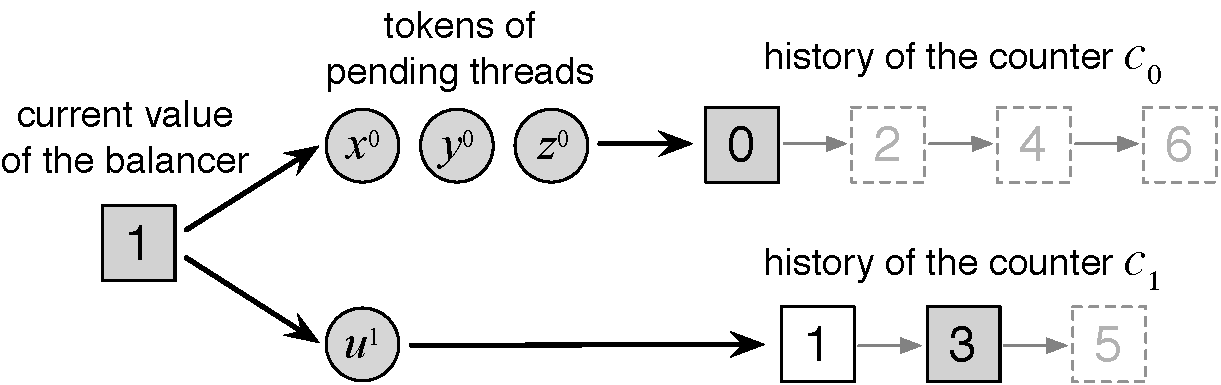
\includegraphics[width=8.2cm]{chist.pdf}      
\caption{Tokens and histories of the simple network}
\label{fig:chist}
\end{figure}
}




% We next list the invariants that describe the interdependence between
% the various components of the real and auxiliary state. 

In addition to $\tkn$ and $\hist$ which come in flavors private to
\emph{self} and \emph{other} threads, we require the following shared
variables: (1) $\heapj$ for the joint heap of the network, and (2)
$b_\joint$, $n^0_\joint$ and $n^1_\joint$ for the contents of $\bal$,
$c_o$ and $c_1$, respectively.

\paragraph{Invariants of the counting network}
\label{sec:count-netw-invar}

The main invariant of the network relates the number of tokens, the
size of histories and the value of the balancer:

\[
\tag{\normalsize{\arabic{tags}}}\refstepcounter{tags}\label{cn:si} 
%
|\hist^0| + |\tkn^0| =
|\hist^1| + |\tkn^1| + b_\joint
\]

The equation formalizes the intuition that out-of-order anomalies of
the counting network appear if one of the two counters is too far
ahead of the other one.
%
The invariant~(\ref{cn:si}) provides a bound on such a situation. One
counter can get ahead temporarily, but then there must be a number of
threads waiting to spend their tokens on the other counter. Thus, the
other counter will eventually catch up.

The approaches such as quiescent and quantitative quiescent
consistency describe this situation by referring to the number of
\emph{unmatched} call events in an event
history~\cite{Derrick-al:FM14,Jagadeesan-Riely:ICALP14}. In contrast,
we formalize this property via auxiliary state: the sets of tokens
$\tknh$ recorded in the entry for the number $t$ determine the
environment's capability to add new history entries, and thus ``run
ahead'' or ``catch up'' after $t$ has been returned.
%
% Such auxiliary state will let us directly specify the network's
% behavior in the moments of quiescence (\ie,~when $\tkno$ is empty),
% but also \emph{quantitatively} bound the out-of-orderness as a
% function of $\tkno$.
%
The other invariants of the counting network are as follows:
%\vspace{2pt}
\begin{enumerate}[label=(\roman*)]

% %
% \[
% \tag{\normalsize{\arabic{tags}}}\refstepcounter{tags}\label{eq:cn-states} 
% {\small
% \begin{array}{r@{\ }c@{\ }l} 
% {\!\!\!\!\!\!\!\!}W_{\ccon} & \!\eqdef & \exists \tkns~\tkno~ \hists~\histo~b~n_0~n_1\ldot 
% %  
% \qcl \spts (\tkns, \hists)\aand \qcl \opts (\tkno, \histo) 
%   \\[4pt] 
% &\aand & \qcl \jpts \bal \hpts b \hunion c_0 \hpts n_0 \hunion c_1 \hpts n_1   
%  \aand \hvalid~(\hists \hunion \histo)         \\[3pt] 
% &\aand & \SI~\tkn^0~\tkn^1~\hist^0~\hist^1~b ~~~~\aand
%          \CI~\hist^0~\hist^1~n_0~n_1 \\[3pt]  
% &\aand & \TI~\tkn^0~\tkn^1~(\hist^0 \hunion \hist^1)\aand \AI~\hist^0~\hist^1~\tkn^0~\tkn^1~n_0~n_1.
% \end{array}
% }
% \]
%

% where $\hist^i = (\hists \hunion \histo)^i$ and
% $\tkn^i = (\tkns \hunion \tkno)^i$ for $i \in \set{0,1}$.

\item\label{cn:state} $\heapj = \bal \mapsto b_\joint \hunion c_0 \mapsto n^0_\joint
  \hunion c_1 \mapsto n^1_\joint$.

\item\label{cn:hvalid} The histories contain disjoint time-stamps. % (\ie $\hists \hunion \histo$ is always defined);
 
% The state-space invariant $W_{\ccon}$ fixes the auxiliary self/other
% components to be pairs of tokens and histories $(\tkns, \hists)$ and
% $(\tkno, \histo)$, which are held/contributed by the thread and its
% environment, correspondingly. The invarian $\hvalid~(\hists \hunion
% \histo)$ ensures that at any moment 
% %
% The joint part of the state contains the pointers $\bal$, $c_0$ and
% $c_1$, and the relations between all these components are specified by
% the invariants $\SI$, $\CI$, $\TI$ and $\AI$.

\item\label{cn:ci} 
%
  The history $\hist^0$ (resp. $\hist^1$) contains \emph{all} even
  (resp. odd) values in $[0, n^0_\joint]$ (resp. $[1, n^1_\joint]$).
%
%    In other words, the network does not ``skip'' values. 
%
    This ensures that $n^0_\joint$ and $n^1_\joint$ are the last
    time-stamps in $\hist^0$ and $\hist^1$, respectively.

\item\label{cn:ti}  
%
  $\tkn^0$, $\tkn^1$ and $\Tomb~(\hists \hunion \histo)$ contain
  mutually disjoint tokens, where $\Tomb~(t \mapsto (\tknh, z) \hunion
  \hist') = \{z\} \hunion \Tomb~\hist'$, and $\Tomb~\emptyset =
  \emptyset$. In other words, a spent token never appears among the
  ``alive'' ones (\ie, in $\tkn^0 \hunion \tkn^1$).

%As a consequence, $\Tomb~(\hists \hunion \histo)$ is always defined.

\item\label{cn:ti1}
%
  $t \mapsto (\tknh, z) \subseteq \hists \hunion \histo
  \implies z \in \tknh$. \\[-7pt]

\item\label{cn:ai} 
%
For any $t$, $\tknh$, $z$: \\[-7pt]
% 
{\small
  \begin{itemize}
  \item   $t \hpts (\tknh, z) \subseteq \hist^0 \implies t + 2\ |\tknh
    \cap \tkn^0| < n^1_\joint + 2\ |\tknh \cap \tkn^1| + 2$, and \\[-7pt]
  \item
    $t \hpts (\tknh, z) \subseteq \hist^1 \implies t + 2\ |\tknh \cap 
    \tkn^1| < n^0_\joint + 2\ |\tknh \cap \tkn^0|
    + 2$.
  \end{itemize}
}
%
\end{enumerate}
\vspace{5pt}
 
\noindent
The invariant~\ref{cn:ai} provides quantitative information about the
network history by relating the actual ($n^0_\joint$, $n^1_\joint$)
and the past ($t$) counter values, via the current amount of
interference ($\tkn$) and the snapshot interference ($\tknh$).
%
To explain~\ref{cn:ai}, we resort to the intuition provided by the
following equality, which, however, being \emph{not quite valid},
cannot be used as an invariant, as we shall see. Focusing on the
first clause in~\ref{cn:ai}, if
$t \mapsto (\tknh, z) \subseteq \hist^0$, then,
intuitively:
%
%
%\vspace{-5pt}
%
{\small{
\[
t + 2\ |\tknh^0 \setminus \tkn^0 | + 2\ |\tknh \cap \tkn^0| =
n^1_\joint + 2\ |\tknh \cap \tkn^1| + (2 b_\joint - 1)
\]}}
%
% \vspace{-5pt}
%
\noindent
The equality says the following. When $t$ is snapshot from $c_0$ and
placed into the history $\hist^0$, the set of outstanding even tokens
was $\tknh^0$. By the present time, $c_0$ has been increased
$|\tknh^0 \setminus \tkn^0|$ times, each time by $2$, thus
$n^0_\joint = t + 2\ |\tknh^0 \setminus \tkn^0|$. What is left to add
to $c_0$ to reach the \emph{period of quiescence}, when no threads
interfere with us, is $2\ |\tknh \cap \tkn^0|$. Similar reasoning
applies to $c_1$. It is easy to see at the period of quiescence, $c_0$
and $c_1$ differ by $2 b_\joint - 1$; that is, the counter pointed to
by $\bal$ is behind by $1$. However, the equality is invalid, as
$b_\joint$ can be read off only in the present, whereas the
``intuitive'' reasoning behind the equality requires a value of
$b_\joint$ from a quiescent period \emph{in the future}. Hence, in
order to get a valid property, we bound $2 b_\joint - 1$ by 2. For
simplicity, we even further weaken the bounds by dropping
$|\tknh^0 \setminus \tkn^0|$ to obtain~\ref{cn:ai}; as it will turn
out, even such a simpler bound will suffice for proving
\textbf{R1}--\textbf{R3}.

% in Section~\ref{sec:qc-client}.

%As already aparent from our explanation, the invariant gives us a way
%to formally model when the network is in the period of quiescence, as
%required in \textbf{R2}, which we verify in
%Section~\ref{sec:qc-client}.
%%

% \gad{I did not find the equation above ``intuitive'' at all. I think
%   it might be better to give the first part of the explanation and
%   introduce the equality. Then, say why it doesn't hold and how to fix
%   it to get a valid invariant. I think that would be easier to
%   understand.}
%
% wontfix
%
% \gad{Also, why the quotation marks around equation? Valid or not, it
%   is still an equality.}
%
% won't fix

\paragraph{Allowed changes in the counting network}
\label{sec:count-netw-prot}


The state of the counting network (auxiliary and real) can be changed
in two possible ways by concurrent threads. These changes formalize
the way the atomic operations \code{flip} and \code{fetchAndAdd2} from
Figure~\ref{fig:counter-fig}~(b) work with auxiliary state.
%
\emph{Flipping} alters the bit value $b_\joint$ of $\bal$ to the
complementary one, $1 - b_\joint$.
%
It also generates a token $z$ (of parity $b_\joint$) and stores it
into $\tkns$. The token is fresh, \ie, distinct from all alive and
spent tokens in $\tkns \hunion \tkno \hunion{\Tomb~(\hists
  \hunion \histo)}$.
%
\emph{Incrementation} spends a token $z$ from $\tkns$, and depending
on its $i$, it atomically increases the value $n^i_\joint$ of $c_i$ by
two, while simultaneously removing $z$ from $\tkns$ (thus, the
precondition is that $z \in \tkns$). It also adds the entry
$(n^i_\joint + 2) \hpts (\tkn^0 \hunion \tkn^1, z^i)$ to $\hists$,
thus snapshoting the values of $\tkn^0$ and $\tkn^1$.
%
It is easy to check that both these allowed changes preserve the
state-space invariants~(\ref{cn:si}), \ref{cn:state}--\ref{cn:ai}, and
that their effect on real state (with auxiliary state erased) are
those of \code{flip} and \code{fetchAndAdd2}.

\subsection{Step 2: a Hoare Spec for \texttt{getAndInc}}
\label{sec:spec-gaa}

Figure~\ref{fig:qspec} provides a Hoare-style spec for
\code{getAndInc}, verified in our proof scripts. We use the logical
variable $\ikn$ and its variants to range over token sets, and $\gist$
to range over histories.

\begin{figure}
\[
%
\tag{\normalsize \arabic{tags}}\refstepcounter{tags}\label{eq:qc-spec}
{\small
\!\!\!\!\!\!\!\! 
\begin{array}{c}
  \spec{\!\!
  \begin{array}{c}
    \tkns = \emptyset,
    \hists = \gists,
    \gisto \subseteq \histo,\\[2pt]
    \ikno \subseteq \tkno \hunion (\Tomb~\histo \setminus
    \Tomb~\gisto),
    \Ic{\gisto}{\ikno}
  \end{array}
  \!\!}
  \\\\[-6pt]
  \texttt{getAndInc()}
  % 
  \\[3pt]
  \spec{\!\!\!
  \begin{array}{c}
    \exists \iknh~z \ldot \tkns = \emptyset, 
    \hists = \gists \hunion (\res + 2) \hpts (\iknh, z), 
    \\[2pt]
    \gisto \subseteq \histo, \ikno \subseteq \tkno \hunion (\Tomb~\histo \setminus \Tomb~\gisto), 
    \\[2pt]
    \last~(\gists \hunion \gisto) < 
    \res + 2 + 2~|\iknh \cap \ikno|, 
    \\[2pt]
    \happrox~(\gists \hunion \gisto)~\res~\iknh~z,
     \Ic{\gisto}{\ikno}
  \end{array} 
  \!\!\!} %@\ccon
%
\end{array}
}
\]
\caption{Hoare-style spec of a simple counting network.}
\label{fig:qspec}
\end{figure}



The precondition starts with an empty token set ($\tkns = \emptyset$),
and hence by framing, any set of tokens. The initial self-history
$\hists$ is set to an arbitrary $\gists$.\footnote{Alternatively, we
  could have also taken $\hists = \emptyset$, but the clients will
  require generalizing to $\hists = \gists$ by the FCSL's frame
  rule~\cite{Sergey-al:ESOP15}. To save space and simplify the
  discussion, we immediately frame \wrt the auxiliary $\hists$. Our
  examples do not require such client-side framing \wrt~$\tkns$.} The
precondition records the \emph{other} components of the initial state
as follows. First, $\gisto$ names (a subset of) $\histo$, to make it
stable under interference, as in Section~\ref{sec:overview}. Next, we
use $\ikno$ to name the (subset of) initially live tokens
$\tkno$. However, as $\tkno$ may shrink due to other threads spending
tokens, simply writing $\ikno \subseteq \tkno$ is unstable. Instead,
we write $\ikno \subseteq \tkno \hunion (\Tomb~\histo \setminus
\Tomb~\gisto)$ to account for the tokens spent by other threads as
well. The set $\tkno \hunion (\Tomb~\histo \setminus \Tomb~\gisto)$
only grows under interference, as new live tokens are generated, or
old live tokens are spent, making the inclusion of $\ikno$ stable.
%
Indeed, one cannot take \emph{any} arbitrary $\gisto$ and $\ikno$ to
name the \emph{other} components of the initial state. Therefore, we
constrain these two variables by the invariant $\ic$, that relates
them to the \emph{self-}components of the actual state and to each
other according to the
invariants~\ref{cn:hvalid}--\ref{cn:ai}.\footnote{That is, $\gisto$
  and $\ikno$ take the role of $\histo$ and $\tkno$ in
  invariants~\ref{cn:hvalid}--\ref{cn:ai}, with
  $n^i_\joint = \last~(\hists \hunion \gisto)^i$. The formal
  definition of $\ic$ is in our proof scripts.} This is natural,
since, as we will see in Section~\ref{sec:qclients}, all clients
instantiate $\gisto$ and $\ikno$ with the \emph{other}-components of
the actual pre-state, respecting~\ref{cn:hvalid}--\ref{cn:ai}.

% \gad{$ \ikno \subseteq \tkno \hunion (\Tomb~\histo \setminus
%   \Tomb~\gisto)$ breaks awkwardly across lines.}
% wontfix
%
% \gad{I don't get the parentheses around ``a subset of''. It makes it
%   harder to read the phrases, and after all the full subset is still a
%   subset.}
%
% fixed
%
% \gad{I did not get what $\Ic{\gisto}{\ikno}$ is, even after browsing
%   the spec in the code. Is it too long to define it inline? Does it
%   matter altogether?}
%
%   Yes, it does matter. And, yes, it's too long to define it in
%   prose, as it's boring and comes from the fact that SL-ish notation
%   is not a good fit for binary state-constrining postconditions.
%

The postcondition asserts that the final token set $\tkns$ is also
empty (\ie, the token that \code{getAndInc} generates by \code{flip},
is spent by the end). The history $\hists$ is increased by an entry
$(\res + 2) \hpts (\iknh, z)$, corresponding to writing the value of
the result (plus two) into one of the network's counters, snapshoting
the tokens of that moment into $\iknh$, and spending the token $z$ on
the write. $\gisto$ is a subset of the new value of $\histo$, and
$\ikno$ is a subset of the new value of $\tkno \hunion (\Tomb~\histo
\setminus \Tomb~\gisto)$, by the already discussed stability.

The next inequality describes where the entry for $\res + 2$ is placed
\wrt~the pre-state history $\gist = \gists \hunion \gisto$. $\gist$
may have gaps arising due to out-of-order behavior of the network, and
$\res + 2$ may fill one such gap. However, there is a bound on how far
$\res$ (and hence $\res+2$) may be from the tail of $\gist$. We
express it as a function of $\ikno$ and $\iknh$, derived from the
bounds in~\ref{cn:ai}, taking $\res + 2$ for $t$ and
over-approximating the instant value $n_{\joint}^i$ of the
incremented counter via $\last~(\gists \hunion \gisto)$. The
inequality weakens the invariant~\ref{cn:ai}, making it hold for even
and odd entries by moving $2~|\iknh \cap \ikno^i|$ (for $i = 0,1$) to
the right side of $<$ and joining them, since $\ikno^0 \cap \ikno^1 =
\emptyset$.

% To explain it, let us assume that $\res$ is written into $c_1$ and the
% last entry of $\hist$ (let us call it $t$) was written into
% $c_0$. Then, we have a similar ``equation'' as in the explanation
% in~\ref{cn:ai}:
% \[
% t + 2\ |\ikno^0 \setminus \iknh^0| + 2\ |\iknh^0 \cap \ikno^0| = \res
% + |\iknh^1 \cap \ikno^1| + (2 b_\joint -1)
% \]
% To advance $c_0$ to the moment when $\iknh^0$ and $\iknh^1$ were
% recorded, we need to increase $t$ by $2\ |\ikno^0 \setminus
% \iknh^0|$. After that, to advance both $c_0$ and $c_1$ to a quiescent
% period, we have to spend the tokens in $|\iknh^0 \cap \ikno^0|$ (for
% $c_0$) and $|\iknh^1 \cap \ikno^1|$ (for $c_1$). In the quiescent
% period, $c_0$ and $c_1$ differ by $2 b_\joint - 1$. Moving $|\iknh^0
% \cap \ikno^0|$ to the other side of the equation (while not changing
% the sign), omitting $|\ikno^0 \setminus \iknh^0|$, and bounding the
% value of $2 b_\joint - 1$ from above by $2$, we get:
% \[
% t < \res + 2\ |\iknh^0 \cap \ikno^0| + 2 \ |\iknh^1 \cap \ikno^1| + 2
% \]
% which we use in~(\ref{eq:qc-spec}). Being symmetric in $\ikn^0$ and
% $\ikn^1$, the inequality has the pleasant property that it also holds
% in the other three cases: when $\res$ is written into $c_0$ and $t$
% into $c_1$, and when both $\res$ and $t$ are written into the same
% counter, $c_0$ or $c_1$.

% The predicate $\strapprox$, stated next, summarizes several properties
% of the result and the newly introduced history entry, which will be
% crucial for reasoning about clients in Section~\ref{sec:qclients}:
% %
% \[
% \tag{\normalsize \arabic{tags}}\refstepcounter{tags}\label{eq:strapprox}
% %
% \!\!\!\!
% {\small{
% \begin{array}{l}
% \strapprox~\gists~\gisto~\ikno~m_0~m_1~\res~\iknh^0~\iknh^1~z
% ~\eqdef
% \\[2pt]
% ~~~~~~~~~~~~~~~~~~ \sapprox~\ikno~m_0~m_1~\res~\iknh^0~\iknh^1, \\[2pt]
% ~~~~~~~~~~~~~~~~~~ \happrox~(\gists \hunion \gisto)~\res~\iknh^0~\iknh^1~z,\\[2pt]
% ~~~~~~~~~~~~~~~~~~ \tapprox~(\gists \hunion \gisto)~\iknh^0~\iknh^1~z
% \end{array}
% }}
% \]
% %
% \[
% %
% \tag{\normalsize \arabic{tags}}\refstepcounter{tags}\label{eq:sapprox}
% %
% {\small{
% \begin{array}{l}
% \sapprox~\ikn~m_0~m_1~\res~\iknh^0~\iknh^1 ~\eqdef \\[2pt]
% %
% ~~~~  m_0 < \res + 2 + 2 \times (|\iknh^0 \cap \ikn^0| + |\iknh^1 \cap
%   \ikn^1|), \\[2pt]
% ~~~~ m_1 < \res + 2 + 2 \times (|\iknh^0 \cap \ikn^0| + |\iknh^1 \cap
%   \ikn^1|)
% \end{array}
% \hfill
% }}
% \]
% 

%\noindent
Finally, the predicate $\happrox$ provides more bounds that we will
need in the proofs of the client code's properties.
%
\[ 
%
\tag{\normalsize \arabic{tags}}\refstepcounter{tags}\label{eq:happrox}
%
\!\!\!\!\!
{\small{
\begin{array}{l}
\!\!\!\!
\happrox~\gist~\res~\iknh~z \eqdef \hbox{}
\iknh \subseteq \tkno \hunion (\Tomb~\histo) \hunion
  \set{z},\\[2pt]
~~ \forall t~\ikn \ldot t \hpts (\ikn, -) \subseteq \gist \Rightarrow
  z \notin \ikn,~  t < \res + 2 + 2 \ (|\iknh \cap \ikn|)
\end{array}
}}
\]
%
When instantiated with $\gist = \gists \hunion \gisto$, $\happrox$
says the following. The token set $\iknh$ snapshot when $\res+2$ was
committed to history, is a subset of all the tokens in post-state,
including the live ones ($\tkno$), and spent ones ($\Tomb~\histo
\hunion \{z\}$).
%
Moreover, if $t$ is an entry in $\gist$, with contents $(\ikn, -)$,
then: (1) $z \notin \ikn$, because $z$ is a token generated when
\code{getAndInc} executed \code{flip}. Hence, $z$ is fresh \wrt~any
token-set from the pre-state history $\gist$; and (2) $t$ and $\ikn$
satisfy the same bounds \wrt~$\res+2$, as those described for the last
history entry and~$\ikno$.


%\noindent

%
% \begin{comment}
% \paragraph{Why the spec~\eqref{eq:qc-spec} is stable?}
% \label{sec:why-spec-eqrefeq:qc}

% The stability of the spec we ascribed to \code{getAndInc} follows from
% the following observations. First, all clauses in the pre- and
% postconditions that contsrain only \emph{self}-components of the state
% (\eg, $s.\hists = \gists$ or $\tkns = \emptyset$) are stable, since
% they cannot be affected by interference (which might change only
% \emph{other} and \emph{joint} components), as ensured by FCSL's
% meta-theory.
% %
% Second, the stability of all other clauses that also mention the
% \emph{other} component, follows from their \emph{monotonicity} with
% respect to interference. In particular, the union
% $\tkno \hunion \Tomb~\histo$, appearing also in the definition of
% $\happrox$, can only grow, while the union
% $\ikno \hunion \Tomb~\gisto$ is fixed.
% %
% Finally, the rest of the clauses mentions only values that are not
% components of the state being constrained (\eg, $\ikno$, $\gisto$,
% \etc) and, hence, are also unaffected by interference.
% %
% All these stability arguments are carried out as formal proofs in our
% Coq development, accompanying the paper.
% \end{comment}

\paragraph{How will the spec~\eqref{eq:qc-spec} be used?}

The clause $\hists\,{=}\,\gists \hunion (\res+2)\,{\mapsto}\,-$ of
\eqref{eq:qc-spec}, in conjunction with the invariant~\ref{cn:hvalid},
ensures that any two calls to \code{getAndInc}, sequential or
concurrent, yield different history entries, and hence different
results. This establishes~\textbf{R1}, which we will not discuss
further.

The inequality on $\last~(\gists \hunion \gisto)$ will provide
for~\textbf{R2} in client reasoning. To see how, consider the
particular case when $\ikno$ is empty, \ie, the pre-state is
quiescent. In that case, the intersection with $\iknh$ is empty, and
we can infer that $\res + 2$, is larger than either counter's value in
the pre-state. As we shall see in Section~\ref{sec:qclients}, this
captures the essence of QC.

Finally, the predicate $\happrox$~\eqref{eq:happrox} establishes a
bound for the ``out-of-order'' discrepancy between the result $\res$
and any value $t$ committed to the history \emph{in the past}, via
$2~|\iknh \cap \ikn|$. We will further bound this value using the size
of $\iknh$, and the inclusion $\iknh \subseteq \tkno \hunion
\Tomb~\histo$ from~\eqref{eq:happrox}. These bounds will ultimately
enable us to derive the requirement~\textbf{R3}.

% \gad{ The $\hists \ldots$ clause line-breaks bad.}

% \subsubsection{Specifications of {\code{flip}} and
%   {\code{fetchAndAdd2}}}
% \label{sec:qacts}

% The formal verification of the spec~\eqref{eq:qc-spec} follows by
% sequential composition of its operations, \code{flip} and
% \code{fetchAndAdd2}, to which we ascribe the following specs.
% %
% Both specs are obtained by relaxing the definitions of the transitions
% from Section~\ref{sec:count-netw-prot}, \wrt~stability.
% %
% %
% \[
% %
% %\tag{\normalsize \arabic{tags}}\refstepcounter{tags}\label{eq:flip-spec}
% {\small
% %\!\!\!\!\!\!\!\! 
% \begin{array}{c}
%   \spec{\!\!
%   \begin{array}{c}
%     \tkns = \emptyset,
%     \hists = \gists,
%     \gisto \subseteq \histo,\\[2pt]
%     \ikno  \subseteq \tkno \hunion (\Tomb~\histo \setminus
%     \Tomb~\gisto), 
%      \Ic{\gisto}{\ikno}
%   \end{array}
%   \!\!}
%   \\\\[-6pt]
%   \texttt{flip(}\bal\texttt{)}
%   %  
%   \\[3pt]
%   \spec{\!\!
%   \begin{array}{c}
%     \exists b~z^b \ldot \res = (b, z^b)\aand
%     \tkns = \set{z^b}\aand \hists = \gists \aand
%      \Ic{\gisto}{\ikno},
%    \\[2pt]
%     \gisto \subseteq \histo, \ikno \subseteq \tkno \hunion (\Tomb~\histo \setminus \Tomb~\gisto),\\[2pt]    
%     \forall t~\ikn^0~\ikn^1 \ldot
%     t \hpts (\ikn^0, \ikn^1, -) \subseteq (\gists \hunion \gisto) \Rightarrow z^b \notin \ikn^0 \hunion \ikn^1,
%     \\[2pt]     
%     \bapprox~(\last~(\gists \hunion \gisto)^0)~(\last~(\gists \hunion \gisto)^1)~\ikno 
%   \end{array}
%   \!\!}@\ccon
% %
% \end{array}
% }
% \]

% \noindent
% The precondition of \code{flip}'s matches the one of
% \code{getAndInc}. The postcondition contains a clause with a new
% predicate $\bapprox$, relating the last entries $m_0$ and $m_1$ of
% either parity of the initial history $\gist = \gists \hunion \gisto$,
% to the current values $n_\joint^0$ and $n_\joint^1$ of $c_0$ and
% $c_1$.
% %
% \[
% %
% \!\!\!\!
% {\small{
% \begin{array}{l}
% \bapprox~m_0~m_1~\ikno \eqdef \\[2pt]
% %
%   \begin{array}{l}
%    m_0 \le n_\joint^0\aand
%     m_1 + 2 \times |\ikno^1 \cap \tkn^1| < n_\joint^0 + 2 \times
%   |\ikn^0 \cap  \tkn^0| + 2, \\[2pt]
%    m_1 \le n_\joint^1\aand m_0 + 2 \times |\ikno^0 \cap \tkn^0| < n_\joint^1 + 2 \times
%   |\ikn^1 \cap  \tkn^1| + 2 
%   \end{array}
% \end{array}
% \hfill
% }}
% \]
% %
% The predicate says that the contents of $c_0$ and $c_1$ increases,
% hence $m_0$ and $m_1$ are smaller or equal to the current values
% $n_\joint^0$ and $n_\joint^1$, respectively. Moreover, when comparing
% values of different parities (\ie, $m_1$ with $n_\joint^0$ and $m_0$
% with $n_\joint^1$), we require bounds similar to the ones already
% discussed in~\ref{cn:ai} and~\eqref{eq:qc-spec}, and expressed in
% terms of token set $\ikno$ and $\tkn = \tkns \hunion \tkno$, that
% capture the interference in the pre-state and post-state,
% respectively. The predicate is internal to \esc{getAndInc}, and is not
% used by, or even visible to, the clients.

% The precondition of \code{fetchAndAdd2} is the same as \code{flip}'s
% postcondition, and \code{fetchAndAdd2}'s post is the one of
% \code{getAndInc}, so verifying the sequential composition is
% straightforward.
% %
% % We note that the $\bapprox$ property is essential for deriving the
% % inequalities from the postcondition~\eqref{eq:qc-spec}.
% %
% \[
% %
% %\tag{\normalsize \arabic{tags}}\refstepcounter{tags}\label{eq:add-spec}
% {\small
% %\!\!\!\!\!\!\!\!\!\! 
% \begin{array}{c}
%   \spec{\!\!
%   \begin{array}{c}
%    \tkns = \set{z^b}\aand \hists = \gists, 
%      \Ic{\gisto}{\ikno} \aand   \\[2pt]
%     \gisto \subseteq \histo, \ikno  \subseteq \tkno \hunion (\Tomb~\histo \setminus \Tomb~\gisto),\\[2pt]
%     \forall t~\ikn^0~\ikn^1 \ldot
%     t \hpts (\ikn^0, \ikn^1, -) \subseteq (\gists \hunion \gisto) \Rightarrow z^b \notin \ikn^0 \hunion \ikn^1,
%     \\[2pt]    
%     \bapprox~(\last~(\gists \hunion \gisto)^0)~(\last~(\gists \hunion \gisto)^1)~\ikno 
%   \end{array}
%   \!\!}
%   \\\\[-5pt]
%   \texttt{fetchAndAdd2($c_b, \specK{z^b}$)} 
%   % 
%   \\[3pt]
%   {\normalsize{ 
%   \specK{\{}~ {\small\texttt{getAndInc}}\specK{\text{'s post~\eqref{eq:qc-spec},
%   instantiated with}~\gists, \ikno, \gisto\}}@\ccon
%   }}
% %
% \end{array}
% }
% \]

% \noindent
% We note one peculiarity, however. In order to provide a provable spec
% for \code{fetchAndAdd2}, we had to augment its signature with a
% \emph{logical} parameter $\specK{z^b}$, representing the token,
% obtained by executing \code{flip}, to be spent in incrementation of
% $c_b$. While in most Hoare-style specs, logical variables scope over
% the precondition and the postcondition, but do not appear in the code,
% here we had to pass $z^b$ as a function argument.
% %
% This logical parameter serves purely for verification purposes, and
% does not affect the result of the execution. Hence, in principle, it
% can be safely erased, though our current formalization of FCSL in Coq
% does not support such erasure.


